
\chapter{Einleitung}
\thispagestyle{fancy}

\begin{quote}
In the spirit of Alfred Nobel the Prize rewards an invention of greatest benefit to mankind; using blue LEDs, white Light can be created in a new way.\end{quote}
\noindent
Dieser Satz, den die Schwedische Akademie der Künste nach der Vergabe des Nobelpreises an die Entwicklung der blauen LED(kurz, light emitting diode) im Jahr 2014 an die Presse veröffentlichte, fasst treffend zusammen, wie hoch die Bedeutung der auf Halbleiterkristallen basierenden optischen Bauelemente ist . LEDs nehmen einen fundamentalen und immer bedeutender werdenden Teil unseres alltäglichen Lebens ein. Ausgezeichnet durch ihre hervorragende Effizienz, konkurrenzlosen Lebensdauer und geringen Dimension übernimmt sie durch eine immer höher werdenden Lichtausbeute zusehends neue Anwendungsbereiche. Insbesondere auf Gallium Nitrid (GaN) basierende Halbleitermaterialien haben einen bahnbrechenden Weg hingelegt, der zur Entwicklung von hoch effizienten und leuchtstarken blauen LEDs führte und ebenfalls Grundlage für die Entwicklung in andere hochenergetische Wellenlängenbereiche darstellt~\cite{risk}. So ebnet GaN auch den Weg für die Erzeugung von ultraviolet emittierenden Leuchtdioden. Der ultraviolette Spektralbereich, der sich unterteilt in den UV-A (400 nm bis 320 nm), UV-B (320 nm bis 280) und UV-C Bereich (280 nm bis 200 nm) ist bedeutend für eine sehr hohe Anzahl spezieller Anwendungsbereiche. Beispielsweise bieten sich UV-LEDs an die bisher für Wasseraufbereitung genutzten Quecksilberdampflampen zu ersetzen, für deren Betrieb Hochspannungsnetzteile verwendet werden, die einen mobilen Einsatz erheblich erschweren können. Hier könnten UV-LEDs Abhilfe verschaffen, die durch ihr kleines Format und durch die niedrigen Betriebsspannungen einen Mobileneinsatz ermöglichen. Ein weiteres Anwendungsgebiet ist die industrielle Aushärtung/Aufbrechung von Lacken und die Gasdetektion. 
\begin{figure}[htb]
    \centering
    \begin{minipage}[t]{0.49\linewidth}
        \centering
        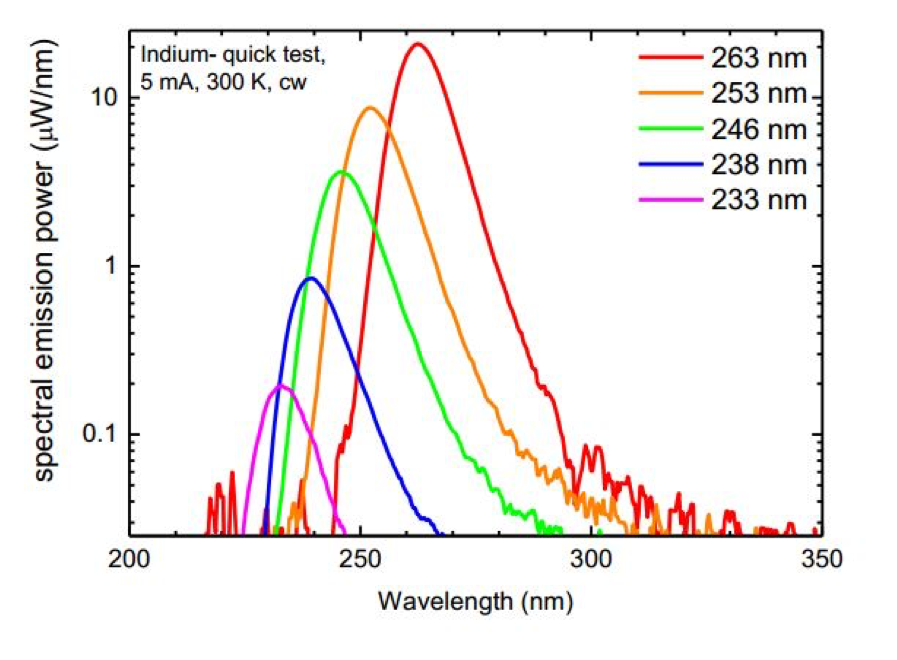
\includegraphics[width=\linewidth]{Bilder/SpectralEmissionPower_Wavelength.png}
        \caption{Spektrable Emissionsleistung für 5 verschiedene Wellenlängen von 263 nm bis 233 nm. Die Grafik zeigt, dass die spektrale Emissionsleistung mit sinkender Wellenlänge ebenfalls sinkt\cite{semreich}.}
        \label{fig:specPowWVL}
    \end{minipage}
    \hfill
    \begin{minipage}[t]{0.49\linewidth}
        \centering
        \includegraphics[width=\linewidth]{Bilder/Schichten.png}
        \caption{Aufbau einer LED-Heterostruktur mit vielen Schichten die unterschiedlichen Zwecken dienen.}
        \label{fig:schichtenLED}
    \end{minipage}
\end{figure}
\vspace{1cm}
\noindent
Für all diese möglichen Applikation ist eine hohe Ausgangsleistung notwendig. Aber wie in Abb. [~\ref{fig:specPowWVL}] zu sehen ist, sinkt die spektrale Emissionsleistung mit kleiner werdendem Wellenlängenbereich signifikant. Der Grund dafür ist, dass UV-LEDs an einer geringen Effizienz leiden, die quantitativ ausgedrückt wird als Externe Quanteneffizienz (EQE) und sich zusammensetzt aus dem Produkt der internen Quanteneffizenz (IQE), Extraktions Effizenz (EE) und Injektionseffizenz(INJ):
%
\begin{equation}
    EQE = IQE \cdot EE \cdot INJ
\end{equation}
%
Die Gründe für die geringe Effizenz sind vielfältig. LEDs bestehen aus einer Vielzahl an Schichten (Abb. [\ref{fig:schichtenLED}]), die unterschiedlichen Funktionen dienen. Diese Schichten werden auf Substraten aufgewachsen. Eine hohe Substratqualität ist also der Grundbaustein für die optischen Eigenschaften und damit besonders entscheidend. Denn eine geringe Defektdichte im Substrat geht einher mit einer ebenfalls geringen Defektdichte in den aufgewachsenen Schichten und damit insbesondere der aktiven Zone, in der Elektronen und Löcher rekombinieren und Licht emittiert wird. Ein weiteres Problem im Zusammenhang mit den geringen Defektdichten, ist ein Mangel an geeigneten Substratmaterialien. So wird aufgrund des Mangels an AlN-Substraten, beruhend auf den Schwierigkeiten bei der Herstellung, auf Saphir Substrate ausgewichen. Diese sind im fernen UV transparent und zusätzlich in großen Mengen in guter Qualität hergestellbar.Problematisch jedoch ist die hohe Gitterfehlanpassung durch die relativ großen Unterschiede zwischen den Gitterkonstanten von AlN/GaN und Saphir.Durch diese, sind AlN- und AlGaN-Schichten nicht vollverspannt aufwachsbar. Das führt dazu, dass die Schichten relaxieren, weil die Elastitzät der Schicht nicht groß genug im Vergleich zur Verspannungsenergie ist. Die Relaxation führt zur Entstehung von Versetzungen und Rissen. Diese agieren im Kristall als sogenannte nicht-radiative Rekombinationszentren die die 
IQE verringern. Die Hauptthematik dieser Arbeit liegt in der  Bestimmung der IQE von AlGaN - Heterostrukturen mit Hilfe von temperaturabhängigen Photolumineszenzmessungen. So lässt sich, bei der Annahme, dass bei Tieftemperatur keine nicht-strahlende Rekombination stattfindet, die IQE als Quotient der Intensität der Photolumineszenz bei Tieftemperatur (5K) und Raumtemperatur (300K) beschreiben. Im Rahmen der Arbeit wird auch eine Methode analysiert, laut der es möglich ist, allein durch leistungsdichteabhängige Messungen bei Raumtemperatur die IQE zu bestimmen. Das ist in so fern ein Vorteil, dass ein aufwändiges Runter kühlen auf 5K nicht notwendig ist. 














